\documentclass{article}
\usepackage[a4paper, left=0.5in, right=0.5in, top=0.5in, bottom=0.5in]{geometry}
\usepackage{graphicx}
\usepackage{float}
\usepackage{caption}

\usepackage{hyperref}
\begin{document}

\section*{SingleCycleImplementation}
\begin{figure}[H]
    \begin{center}
        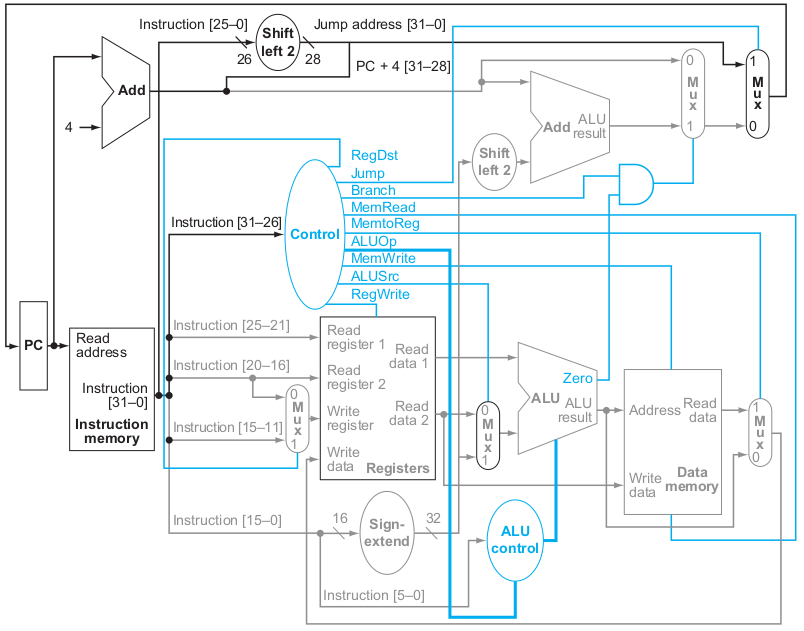
\includegraphics[scale=0.5]{SingleCycleImplementation/SingleCycle.png}
        \caption*{FIGURE 4.24 The simple control and datapath are extended to handle the jump instruction.}
    \end{center}
\end{figure}


\begin{itemize}
    \item Single Cycle
    \item No pipelining
    \item Not Synthesizable
    \item Supports \verb|add|, \verb|sub|, \verb|sw|, \verb|ld|, \verb|beq| and \verb|b|.
\end{itemize}


\section*{PipelinedImplementation1}
\subsection*{Project 1}
\begin{figure}[H]
    \begin{center}
        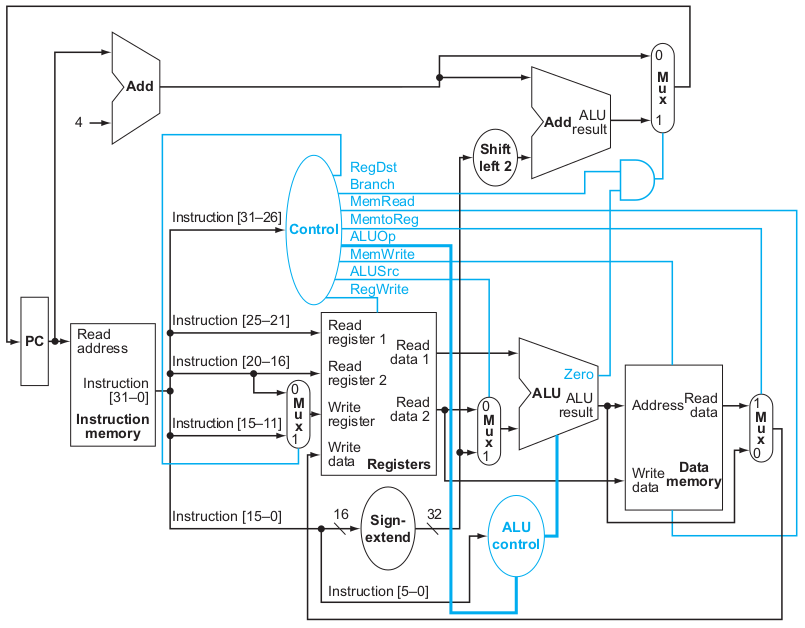
\includegraphics[scale=0.5]{PipelinedImplementation1/Implementation1_pro1.png}
        \caption*{FIGURE 4.17 The simple datapath with the control unit.}
    \end{center}
\end{figure}

\begin{itemize}
    \item Single Cycle
    \item Simple Pipelined
    \item Synthesizable
    \item Supports \verb|add|, \verb|sub|, \verb|sw|, \verb|ld| and \verb|beq|.
    \item No Hazard Mangement.
\end{itemize}

\subsection*{Project 2}
\begin{figure}[H]
    \begin{center}
        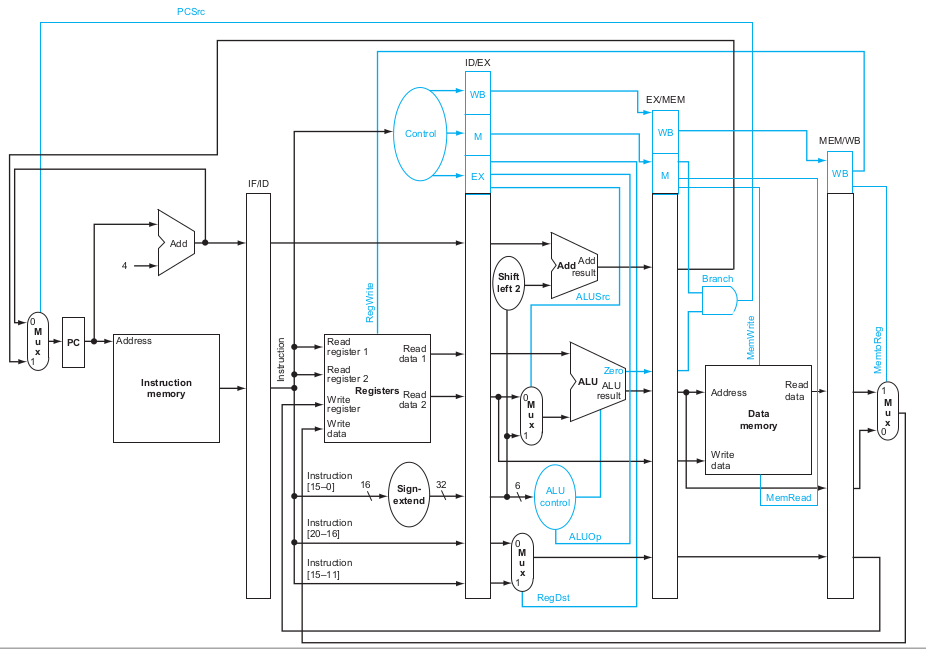
\includegraphics[scale=0.5]{PipelinedImplementation1/Implementation1_pro2.png}
        \caption*{FIGURE 4.51 The pipelined datapath of Figure 4.46, with the control signals connected to the control portions of the pipeline registers.}
    \end{center}
\end{figure}

\begin{itemize}
    \item Single Cycle
    \item Simple Pipelined (same as Project 1 but with seperate blocks)
    \item Synthesizable
    \item Supports \verb|add|, \verb|sub|, \verb|sw|, \verb|ld| and \verb|beq|.
    \item No Hazard Mangement.
\end{itemize}

\section*{PipelinedImplementation2}
\begin{figure}[H]
    \begin{center}
        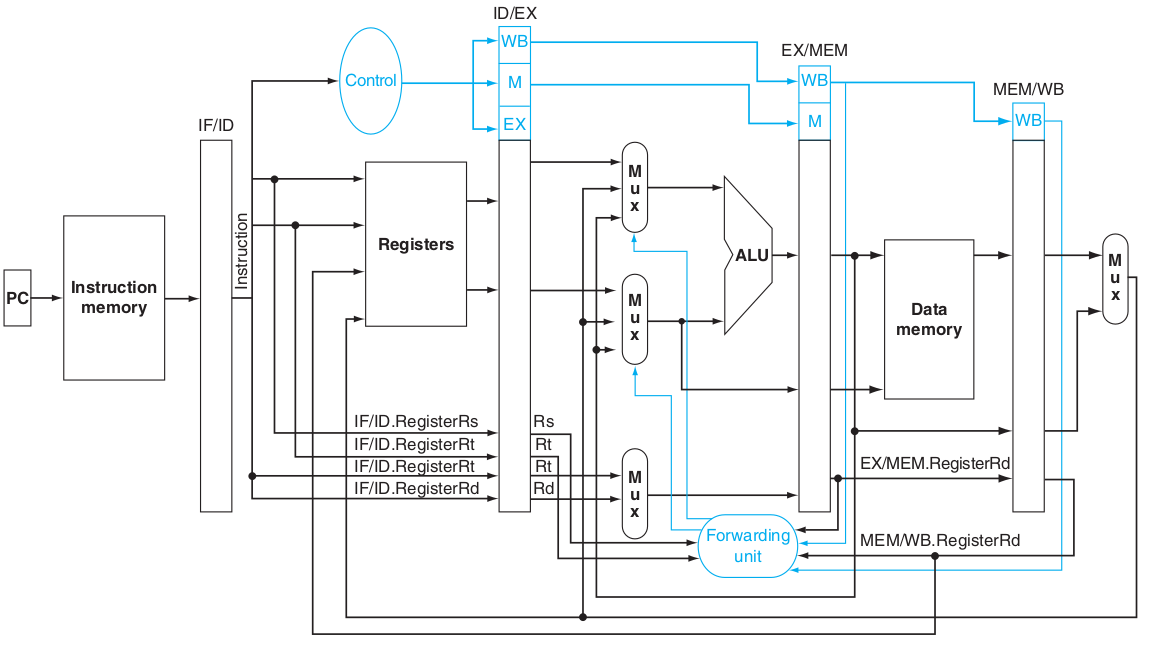
\includegraphics[scale=0.4]{PipelinedImplementation2/PipelinedVersion_Forwarding.png}
        \caption*{FIGURE 4.56 The datapath modifi ed to resolve hazards via forwarding.}
    \end{center}
\end{figure}
\begin{figure}[H]
    \begin{center}
        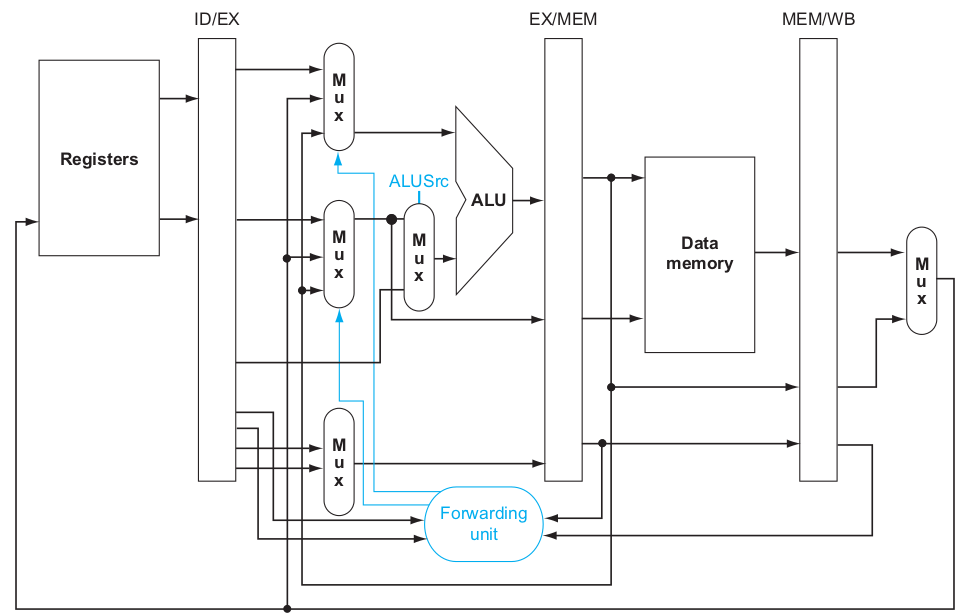
\includegraphics[scale=0.5]{PipelinedImplementation2/PipelinedVerson_Forward2.png}
        \caption*{FIGURE 4.57 A close-up of the datapath in Figure 4.54 shows a 2:1 multiplexor, which has been added to select the signed immediate as an ALU input.}
    \end{center}
\end{figure}

\begin{itemize}
    \item Single Cycle
    \item Piplined with Forwarding for Data Hazard
    \item Synthesizable
    \item Supports \verb|add|, \verb|sub|, \verb|sw|, \verb|ld| and \verb|beq|.
    \item Data Hazard between stages (see below).
          \begin{figure}[H]
              \begin{center}
                  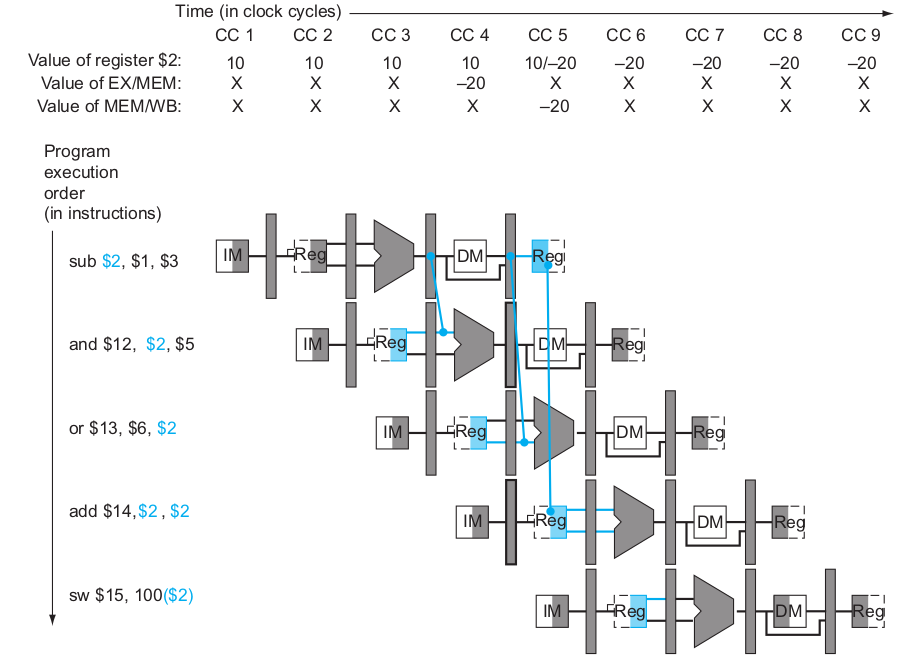
\includegraphics[scale=0.5]{PipelinedImplementation2/PipelineingEg.png}
                  \caption*{FIGURE 4.53 The dependences between the pipeline registers move forward in time, so it is possible to supply the inputs to the ALU needed by the AND instruction and OR instruction by forwarding the results found in the pipeline registers}
              \end{center}
          \end{figure}
    \item Also, added another forwarding(see below) from writeback to execution.
          \begin{figure}[H]
              \begin{center}
                  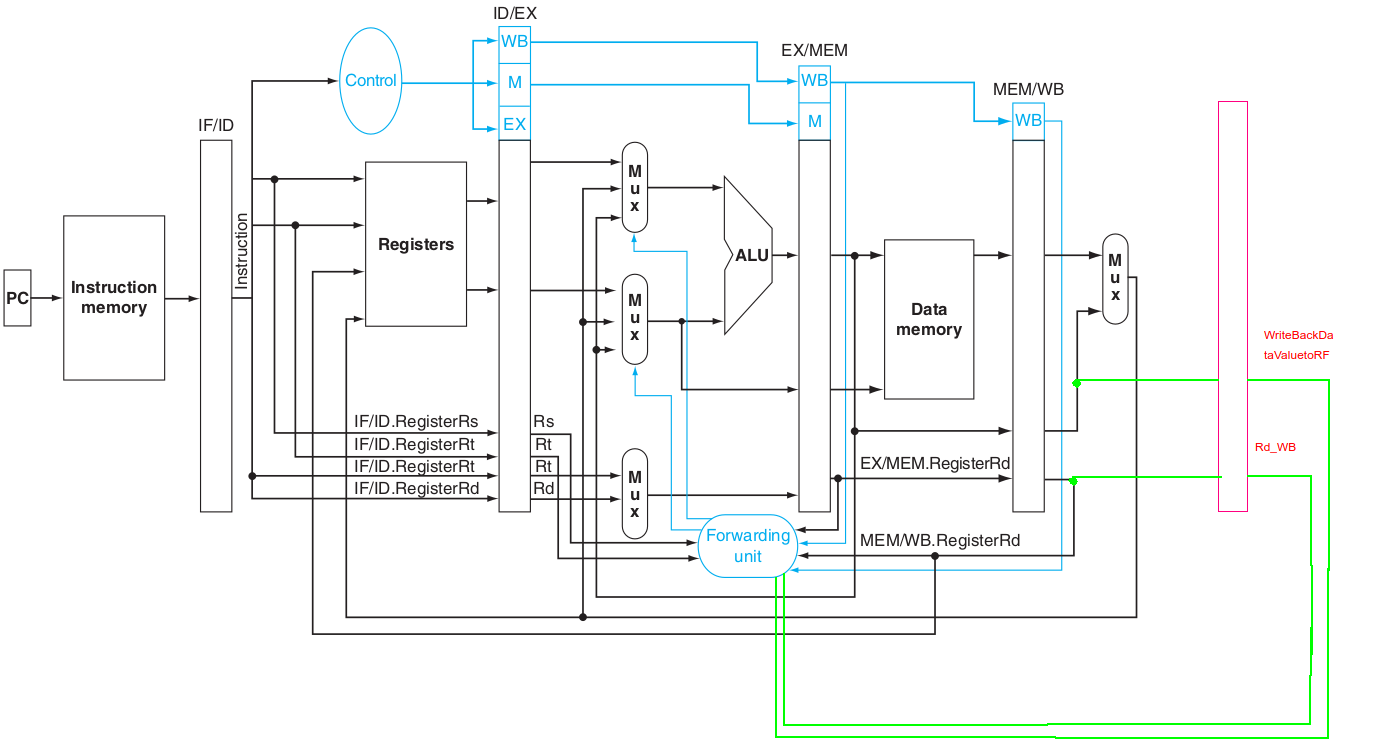
\includegraphics[scale=0.35]{PipelinedImplementation2/PipelinedVersion_Forwarding_Mod.png}
              \end{center}
          \end{figure}
\end{itemize}
\section*{Note}
\quad Left till forwarding in \textbf{Computer Organization and Design MIPS Edition The HardwareSoftware Interface (The Morgan Kaufmann Series in Computer Architecture and Design) by David A. Patterson, John L. Hennessy (z-lib.org).pdf} - Haven't implemented stallls - Pg no. 313.



\section*{MultiCycleImplementation}

\subsection*{Project 1}
\begin{figure}[H]
    \begin{center}
        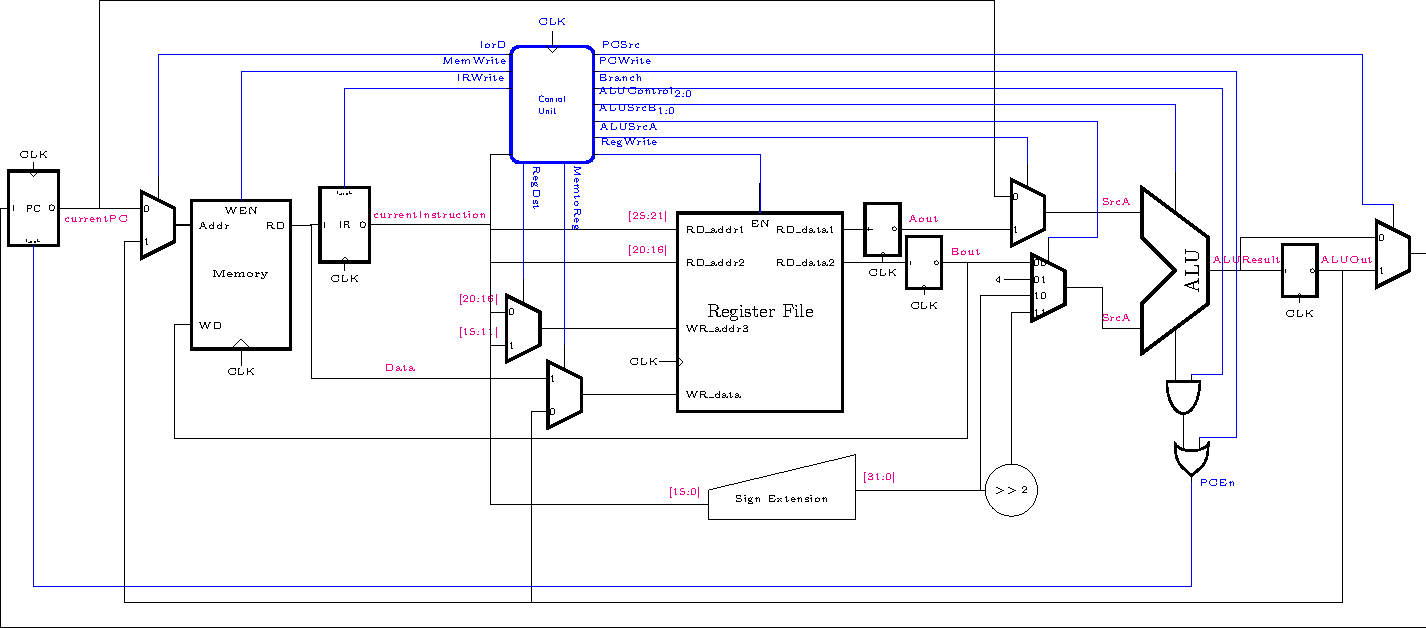
\includegraphics[scale=0.75]{MultiCycleImplementation/TexFiles/MultiCycle1.pdf}
        \caption*{\textbf{Removed the Data register as already data's are registerd from memory}}
    \end{center}
\end{figure}


\begin{itemize}
    \item Multi Cycle
    \item No data Hazard
    \item No Control Hazard
    \item Synthesizable
    \item Supports \verb|add|, \verb|sub|, \verb|sw|, \verb|ld| and \verb|beq|.
    \item Uses FSM
    \item Shrinked from Single Cycle
\end{itemize}

\subsubsection*{State Diagram}
\begin{figure}[H]
    \begin{center}
        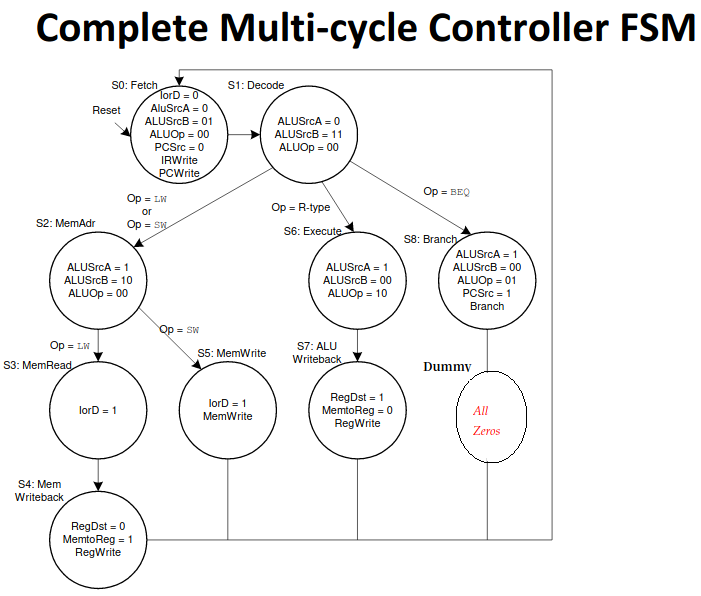
\includegraphics[scale=0.5]{MultiCycleImplementation/MIPsMulticylce_FSM.png}
        \caption*{\textbf{Added a new dummy state for }\textit|beq|}
    \end{center}
\end{figure}




\subsection*{Project 2}
\begin{figure}[H]
    \begin{center}
        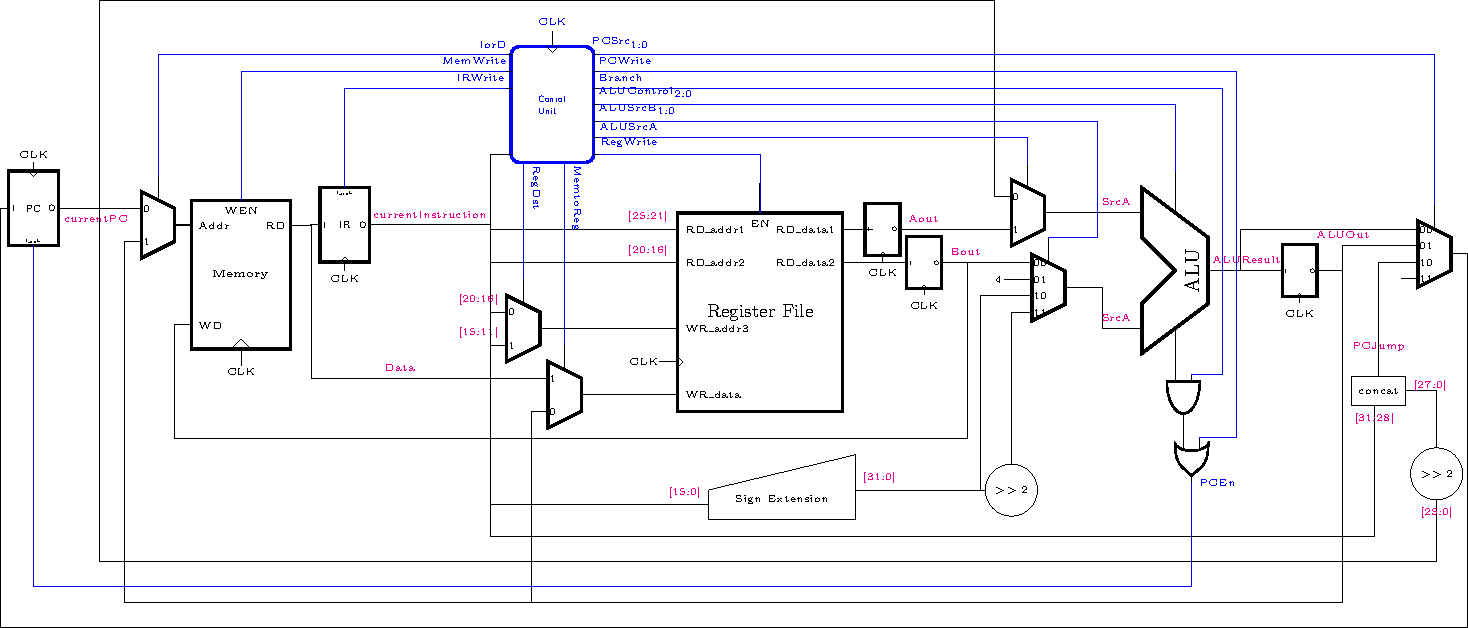
\includegraphics[scale=0.74]{MultiCycleImplementation/TexFiles/MultiCycle2.pdf}
        \caption*{\textbf{added Support for Jump instruction}}
    \end{center}
\end{figure}
\begin{itemize}
    \item Multi Cycle
    \item No data Hazard
    \item No Control Hazard
    \item Synthesizable
    \item Supports \verb|add|, \verb|sub|, \verb|sw|, \verb|ld|, \verb|beq| and \verb|j|.
    \item Uses FSM
    \item Shrinked from Single Cycle
\end{itemize}
\subsubsection*{State Diagram}
\begin{figure}[H]
    \begin{center}
        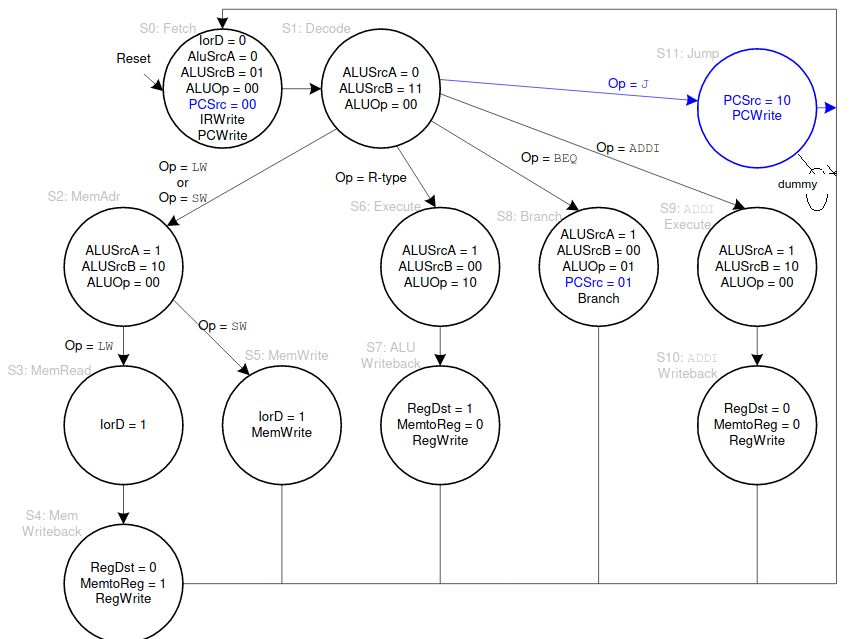
\includegraphics[scale=0.5]{MultiCycleImplementation/MISPImplementationFSM_JUMP.png}
        \caption*{\textbf{Added a new dummy state for }\textit|j|}
    \end{center}
\end{figure}


\subsection*{Project 3}

\begin{itemize}
    \item Multi Cycle
    \item No data Hazard
    \item No Control Hazard
    \item Synthesizable
    \item Supports \verb|add|, \verb|sub|, \verb|sw|, \verb|ld|, \verb|beq|,\verb|j| and \verb|addi|.
    \item Uses FSM
    \item Shrinked from Single Cycle
\end{itemize}
\subsubsection*{State Diagram}
\begin{figure}[H]
    \begin{center}
        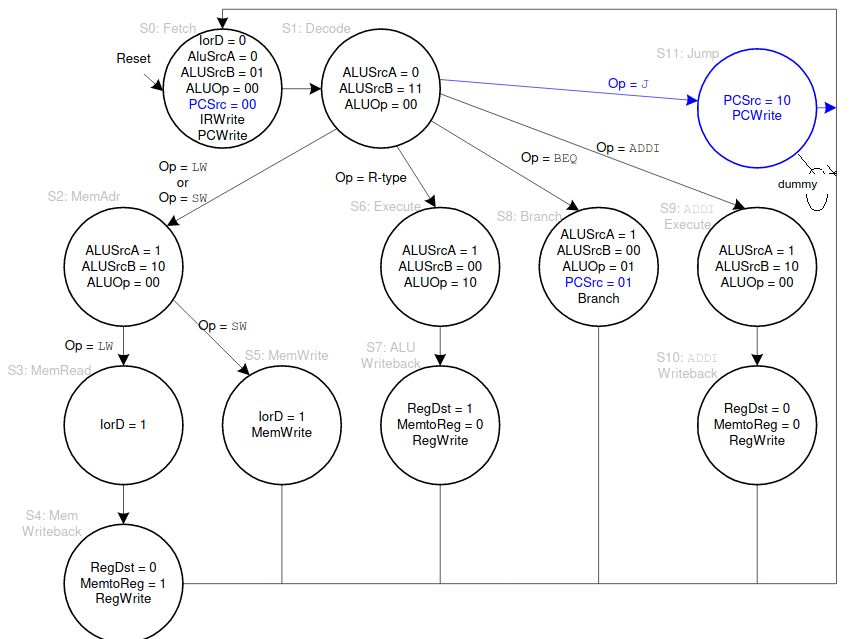
\includegraphics[scale=0.5]{MultiCycleImplementation/MISPImplementationFSM_JUMP.png}
    \end{center}
\end{figure}


\subsection*{References}
\begin{itemize}
    \item \href{https://syssec.ethz.ch/content/dam/ethz/special-interest/infk/inst-infsec/system-security-group-dam/education/Digitaltechnik_14/21_Architecture_MultiCycle.pdf}{L1}
    \item \href{https://nptel.ac.in/courses/106/102/106102062/#downloads}{L2}
    \item \href{https://www.cs.fsu.edu/~zwang/files/cda3101/Fall2017/Lecture6_cda3101.pdf}{L3}
\end{itemize}


\section*{MultiCycleImplementation\_NewOnes}
\subsection*{Project 1}

\begin{itemize}
    \item Added support for "and, or, nor".
\end{itemize}

\subsection*{Project 2}
\begin{figure}[H]
    \begin{center}
        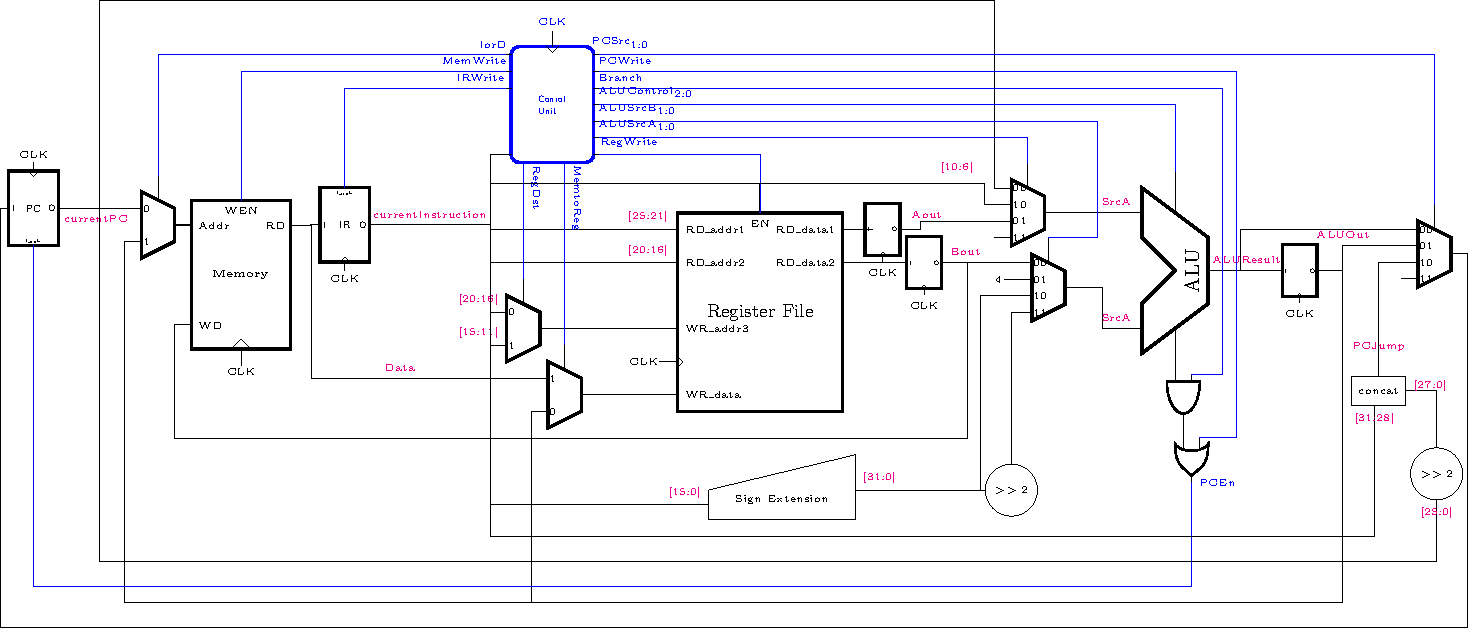
\includegraphics[scale=0.7]{MultiCycleImplementation_NewOnes/TexFiles/MultiCylcle_NewOnes2.pdf}
        \caption*{Changed ALUsrc A Mux}
    \end{center}
\end{figure}
\begin{itemize}
    \item Modified controller FSM add immediate to general immediate.
    \item Modified DataPath to have shfit based operation (ALU is included with shift operations with operand reversed).
    \item Replaced 2x1 mux of ALUSrcA with 4x1 mux with the third input being the 5bit value of immediate.
    \item Modified controller FSM to incorporate shift operation with R type instruction.
    \item Added support for "addi, andi, ori, sll and srl".
\end{itemize}

\subsection*{Project 3}
\begin{figure}[H]
    \begin{center}
        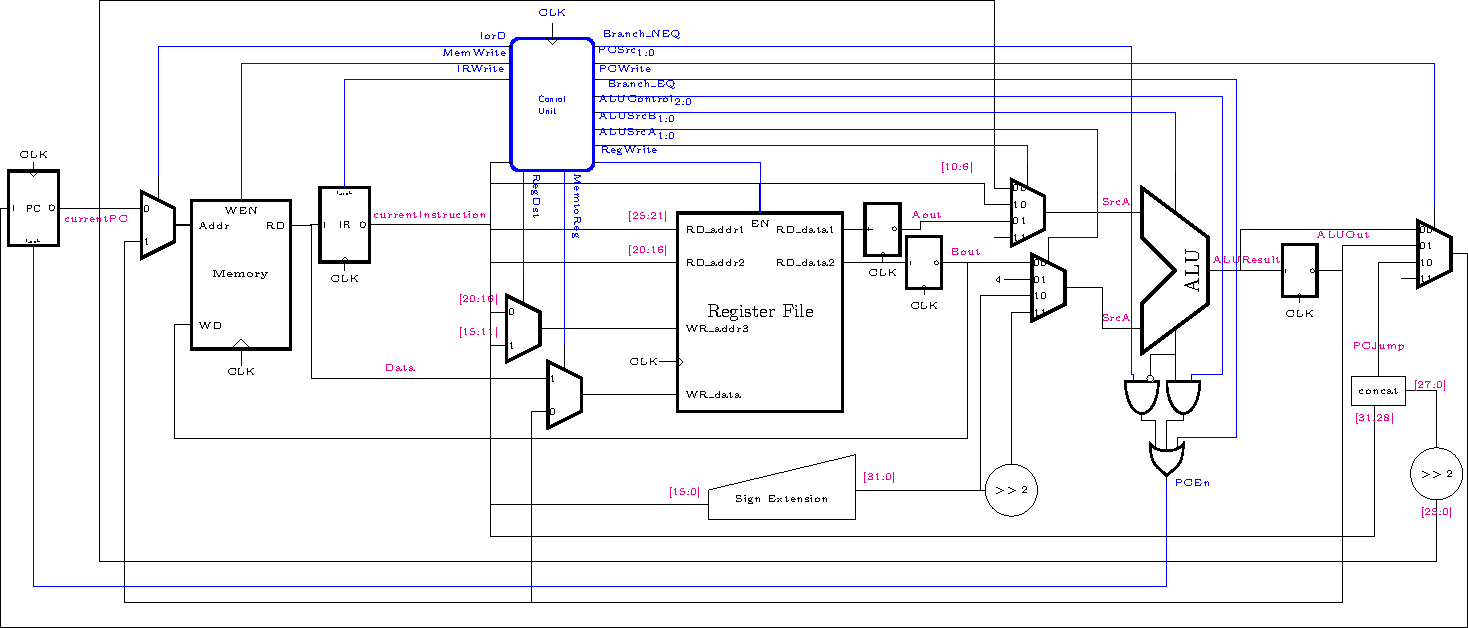
\includegraphics[scale=0.7]{MultiCycleImplementation_NewOnes/TexFiles/MultiCycle_NewOnes3.pdf}
        \caption*{Added support for bneq}
    \end{center}
\end{figure}
\begin{itemize}
    \item Modified Data Path to incorporate "bne" by adding Branch\_neq signal form controller and AND with $\overline{isZero}$ which is ORred with PCWrite.
    \item Modifed FSM to have both "beq" and "bne" in same \verb|BRANCH| state.
\end{itemize}

\end{document}